%%%%%%%%%%%%%%%%%%%%%%%%%%%%%%%%%%%%%%%%%%%%%%%%%%%%%%%%%%%%%%%%%%% 
%                                                                 %
%                            CHAPTER FOUR                        %
%                                                                 %
%%%%%%%%%%%%%%%%%%%%%%%%%%%%%%%%%%%%%%%%%%%%%%%%%%%%%%%%%%%%%%%%%%% 
 
\chapter{Numerical Tests}

In this chapter, we test the Homotopy RSNK optimization algorithm and the preconditioners 
on two constructed analytical problems to investigate the algorithm's non-convexity 
handling capacity and scalability performance. The first one is a constructed indefinite 
quadratic problem with bound constraints. The second one is a constructed convex 
quadratic problem with linear inequality constraints. The second problem is scalable with 
the problem dimension ranges from 100 to 500. A state-of-the-art optimization package 
SNOPT is benchmarked with on accuracy and scalability performance.   

\section{General Information for Test Problems}
\subsection{Optimization Environment - Kona}\label{sec:kona_mv}
The previously introduced Homotopy RSNK method and the preconditioners are part of 
our in-house optimization package, Kona~\cite{dener:scitech2016}. Kona is a matrix-free, 
parallel agnostic optimization package aiming for solving large-scale PDE-constrained 
optimization problems.  It has implemented several optimization 
algorithms including an unconstrained 
reduced-space quasi-Newton method, an unconstrained reduced-space 
Newton-CG method, an equality constrained reduced-space Newton-Krylov 
based on FLECS~\cite{hicken:flecs2014}, and a composite-step RSNK.    
It contains various types of tools for supporting the functions of the optimization algorithms, e.g. 
iterative matrix-free solvers like FGMRES, STCG, FLECS for the linear systems, 
globalization techniques including trust-region, backtracking line search and line search with 
the strong Wolfe conditions, and merit functions like augmented Lagrangian and $l_2$ 
merit function. Besides, it computes the matrix-vector product of the Hessian of the Lagrangian 
by solving two second-order adjoint systems. 

Architechturally, it separates the optimization algorithms with the optimization 
problem interface, allowing the development of new optimization algorithms independently with 
new problem solvers. From a user's perspective, one has to write a solver interface to Kona providing 
a series of function operations as listed in Table 4.1 in~\cite{dener_thesis_2017}. The solver interface 
functions the same as the objective/constraint function and the sensitivity function in SNOPT, or 
other popular optimization methods like fmincon in Matlab. During the optimization process, 
conventional optimizers will call those functions for evaluating the function values and sensitivities 
values at different design points, then make decisions on where to go for the next point. 
The sensitivities demanded are the total gradients. In presence of state variables for 
PDE-constrained optimization, total gradients are expensive as each one would require an adjoint solve, 
as explained in detail in Chapter~\ref{sec:pde_mot}. In contrast, the structure of the solver interface 
required by Kona is designed specially for PDE-constrained optimization problems by providing 
partial gradients instead of total gradients, and matrix-vector products with the system matrix of 
the PDE solvers, with the Jacobians of the constraints w.r.t. the state variables, and with 
the Jacobians of the constraints w.r.t. the design variables. These matrix-vector products 
with the Jacobians are used to assemble the matrix-vector products with the Lagrangian Hessian 
and the total constraint gradients, which in turn are used by the Krylov solvers to solve the linear systems.    

The Homotopy RSNK method developed in this work is placed together with the other unconstrained 
and equality constrained optimization methods, with the same interface and using the same 
vector and matrix operator modules. The preconditioners are likewise placed in the preconditioned folders. 
When testing different problems, the user will first write the solver interface, then setup the running script 
to execute the optimization. 

Although Homotopy RSNK's strength is in PDE-constrained optimization area in presence of 
state variables, it can still be used on problems without state variables, where the conventional 
optimization methods dominate.  For such problems, the total gradients are usually cheap to 
calculate and readily available. For instance, to solve a linear system involving the total constraint Jacobian, 
conventional optimization methods would ask to compute and 
store these total gradients for once, then find the solution by operating directly to the matrix entries.  
In contrast, when using the Homotopy RSNK method, it would ask to calculate the matrix-vector 
products several times in order to form the Krylov subspace. Each time the constraint Jacobian is 
calculated and multiplied with the incoming vector, then released from the memory space. 
So it's the memory cost of the storage of the matrix versus the computational cost of matrix-vector products 
for several times. For some problems, the matrix exists in the form of basic algebraic operations, saving the memory cost of storing the matrix even for once. 


\subsection{SNOPT}
SNOPT is short for Sparse Nonlinear OPTimizer~\cite{gill:2002}, a gradient-based sequential 
quadratic optimization method for solving large-scale nonlinear optimization problem 
with thousands of constraints and design variables. It uses an augmented Lagrangian 
merit function, and the Hessian of the Lagrangian is approximated
using a limited-memory quasi-Newton method. In this work, we use its Python interface 
pyOpt to compare its performance with that of the proposed Homotopy RSNK method. 
SNOPT uses major feasibility and major optimality to measure the progress of the 
optimization iteration. The feasibility measures the maximum nonlinear constraint violation, 
normalized by the size of the solution,
\begin{equation*}
\text{snopt feasibility} = \underset{i}{\text{max}}  \ \text{viol}_i / \lVert x \rVert 
\end{equation*}
where $\text{viol}_i$ is the violation of the $i$th nonlinear constraint~\cite{snopt_manual}. The feasibility tolerance 
$\epsilon_r$ is predefined, with a default value of $10^{-6}$. If it is known that some of the problem 
functions are of low accuracy, a larger value for the feasibility tolerance is appropriate. 

The optimality measures the maximum complementarity slackness for the design variables, 
and is calculated using the following formulas, 
\begin{equation*}
\text{snopt optimality} = \underset{j}{\text{max}}  \ \text{Comp}_j / \lVert \pi \rVert 
\end{equation*}
where $\text{Comp}_j$ measures the complementarity slackness for $j$th variable and is defined by:
\begin{equation*}
\text{Comp}_j = \begin{cases}
d_j \text{min} (x_j - l_j, 1)  \quad \text{if} \ d_j \geq 0 \\
-d_j \text{min} (u_j - x_j, 1) \quad \text{if} \ d_j < 0
\end{cases}
\end{equation*}
where $d_j = g_j - \pi^T a_j$ is the gradient of the Lagrangian, $g_j$ is the $j$th objective gradient, 
$a_j$ is the $j$th constraint Jacobian, $\pi$ is the dual variables. 

\subsection{Basic Settings for the Algorithm}
To measure the progress of the optimization iterations, we evaluate the infinite
norm of each row block in $F(x)$. Specifically, we will refer to optimality,
complementarity, and feasibility as defined below:
\begin{align*}\label{eq:optfeas}
\text{Optimality} &= \lVert   \nabla_x f(x) + \lambda^T \nabla_x g(x)  \rVert _{\infty} \\
\text{Complementarity} &=  \lVert   -\mat{S}\mat{\Lambda} e   \rVert _{\infty}   \\
\text{Feasibility} &= \begin{Vmatrix} h(x) \\ g(x) - s  \end{Vmatrix} _{\infty} 
\end{align*}

In the following tests, the convergence plots display the above metrics versus
computational cost.  Note that the absolute values of the above metrics are used, 
as the initial complementarity products are zero because of zero initial multipliers, 
and the initial feasibility is zero when we use $s_0 = g(x_0)$ for the inequality-only 
structural problem. 

For simplicity, the convergence plots show only the
predictor points before $\mu$ reaches $\epsilon_\mu$, plus all the corrector
points at the last homotopy iteration when $\mu < \epsilon_{\mu}$.

Table \ref{tab:param} shows the parameters used in the test problems, including
the default values set in the algorithm and the recommended ranges.

\begin{table}[tbp]
  \begin{center}
    \caption{Parameters used in the test problems \label{tab:param}}
  \begin{tabular}{ l c c c c c}
    \textbf{Parameters} & $\textbf{Default}$  & $\textbf{Range}$ & $\textbf{Nonconvex}$ 
    & $ \textbf{Quadratic} $ & \textbf{Structural}  \\ \hline
    %\rule{0ex}{3ex}%
    \multicolumn{6}{ l }{Predictor-Corrector Algorithm} \\   %  $\delta_{\text{targ}}$ and $\phi_{\text{targ}}$. 
    \hline
    $K_{\max}$             	&  100     & $\geq$100         & 100 	 &  100       &    100     \\ 
     $J_{\max}$  		&   2         & $\geq$2         & 2             & 2           &      2        \\
    $\epsilon_F$ 	           		&  1e-6     & [1e-8, 1e-3]   & 1e-7 	 & 1e-7       &    1e-4    \\ 
       $\tau$    		&   0.1      & [0.1,0.5]	        & 0.1          & 0.1	 &     0.1    \\
    $\epsilon_H$    		&   0.1      & [0.1,0.5]	        & 0.1          & 0.1	 &     0.1    \\
    $\epsilon_{\mu} $   & 1e-9     & [1e-10, 1e-6]  &   1e-9  & 1e-9  & 1e-6  \\   
    \textbf{$\alpha_0$}             &  0.05     & $\geq$0.01         & 0.05	 & [40,60,80,100,120]  &  0.05  \\
    $\delta_{\text{targ}}$      &  1.0	& [1.0,10]          & 10		 & 10    &   1.0    \\
    $\phi^{\circ}_{\text{targ}}$   & 10.0	& [5.0,50] 	       & 10		 & 20    &   10     \\
    $\zeta_{\max}$ 		        &  50		& [10,50]	       & 50		 & 50    	 &   50     \\
    $\zeta_{\min}$ 		        &  0.5	& 0.5		       & 0.001	 & 0.001    &   0.5   \\
    $\Delta \mu_{\max}$		        &  -5e-4	& [-5e-4, -5e-1]  & -5e-4	 & -5e-4     &  -5e-4  \\  
    $\Delta \mu_{\min}$		        &  -0.9	& -0.9 	       & -0.9		 & -0.9       &  -0.9    \\
    $s_0$                           & $\mathbf{e}$     &   $>$ 0    &    5$\mathbf{e}$    &  10$\mathbf{e}$   &  $g(x_0)$  \\ 
    $\tau_s$                      & 1e-6    & 1e-6    &  1e-6    &  1e-6    & 1e-6   \\
    \hline
    \multicolumn{6}{ l }{Preconditioner} \\ 
    \hline    
    $\mathbf{{n_{\mat{\Sigma}}}}$    & 5	       & $\geq$2		&  -	         &  2          &  [20,80,320]  \\
    $\beta$				& 1.0	       & $>$0        & -         &  -      &  0.1  \\
    $N_{\text{bfgs}}$		& 10	       & [1, 20]		& - 		 &  10	& -  \\
    $\mu_e$			& -1	       & [0, 1] 		& -	         &  -	        & 1e-3  \\
    $\Sigma_e$			& 1 	       & [0, 1]                 & -		& -		& 1e-3  \\
    \hline
    \multicolumn{6}{ l }{Krylov Iterative Solver} \\ 
    \hline       
    $n_k$		& 20        & [10,30]              & 20		 &  20       &  20  \\
    $\epsilon_{\text{krylov}}$		& 1e-2     & [0, 0.1]           	&1e-2	 &  1e-2    &  1e-4  \\
    \hline
  \end{tabular}
  \end{center}
\end{table}

\section{Non-convex Problem}
\subsection{Problem Description}
We consider the following simple nonconvex optimization problem :
\begin{equation*}
\begin{aligned}
&\underset{x \in R^{100}} {\text{min}}  
& &\phantom{-} \frac{1}{2}x^T \mat{Q} x \\
  & {\text{subject to}}
& &-1 \leq x_i \leq 1 \qquad \forall i = 1,2,\ldots,100 \\
\end{aligned}
\end{equation*}
where the pattern of $\mat{Q} = \textsf{diag}(1,-1,1,\ldots,1,-1)$ is randomly generated. 

This problem is challenging for Newton-based optimization algorithms, which 
tends to locate stationery points where $F(q) = 0$ but cannot differentiate between 
a minimizer or a maximizer. As the objective function can be separated into 
individual dimensions, it is easy to see that the minimizer for this problem has the pattern
corresponding to $\mat{Q}$: 
\begin{equation}\label{eq:pattern}
  x^{*} = \begin{bmatrix} 0 & \pm 1 & 0 & \cdots & 0 & \pm 1 \end{bmatrix}^{T}.
\end{equation}
where
\begin{equation}\label{eq:pattern2}
  \begin{gathered}
  x_i=0  \text{~if~}  \mat{Q}_{ii} = 1  \\
  x_i = \pm 1  \text{~if~}  \mat{Q}_{ii} = -1
  \end{gathered}
\end{equation}
We would like to see 
the ability of the algorithm to bypass the wrong solutions in individual dimensions, e.g. $x_i = 0$ 
when $\mat{Q}_{ii} = -1$ and $x_i = \pm 1$ when $\mat{Q}_{ii} = 1$.
Note that when $\mat{Q}_{ii} = 1$, the upper and lower bound $x_i = \pm 1$ are 
individual maximums where the gradient of the Lagrangian is zero in that dimension. 

\subsection{Results - Nonconvexity}
We ran the optimization algorithm on 1000 random cases. For each case, 
the arrangement of $1$ and $-1$ in $\mat{Q}$ is uniformly randomly generated; 
 the initial point $x_0$ is also generated randomly with uniform probability in the domain
  $\Omega = \{ x \in \mathbb{R}^{100} \; | \; -2 \leq x_i \leq 2 \}$.  We call a solution successful if 
  its pattern is exact as \eqref{eq:pattern2}.  Table~\ref{tab:success} lists the success rate for different 
  combinations of $\epsilon_{\text{krylov}}$ and $\epsilon_F$. 
 
\begin{table}[H]
  \begin{center}
    \caption{Success Rate with Different Parameters \label{tab:success}}
  \begin{tabular}{| c |  c |  c |  c | c | c | c | c |}
  \hline
 & \multicolumn{7}{  c  | }{ $\epsilon_{\text{krylov}}$  } \\  \hline
 &   & 1e-1  & 1e-2    & 1e-3    &  1e-4    &  1e-5   & 1e-6  \\  
\multirow{2}{*}{$\tau$ and $\epsilon_F$ } &  1e-1 & 51\%  &90.0\% &94.2\% &94.6\% &93.9\% & 93.8\%  \\
	               					      &   1e-2 & 47.2\%  &93.1\% &94.4\% &93.9\% &94.2\% &  94.5\%\\
    \hline
  \end{tabular}
  \end{center}
\end{table}

As can be seen from Table~\ref{tab:success}, the robustness of the algorithm for handling non-convexity 
is obviously impacted by the tolerances. It shows that $\epsilon_{\text{krylov}}$ has to be below $1e-2$ 
for effective non-convexity handling ability, and the predictor and corrector linear solve tolerance $\epsilon_F$ 
plays a smaller role than $\epsilon_{\text{krylov}}$.   
  
 \begin{figure}[tbp]
  \centering
  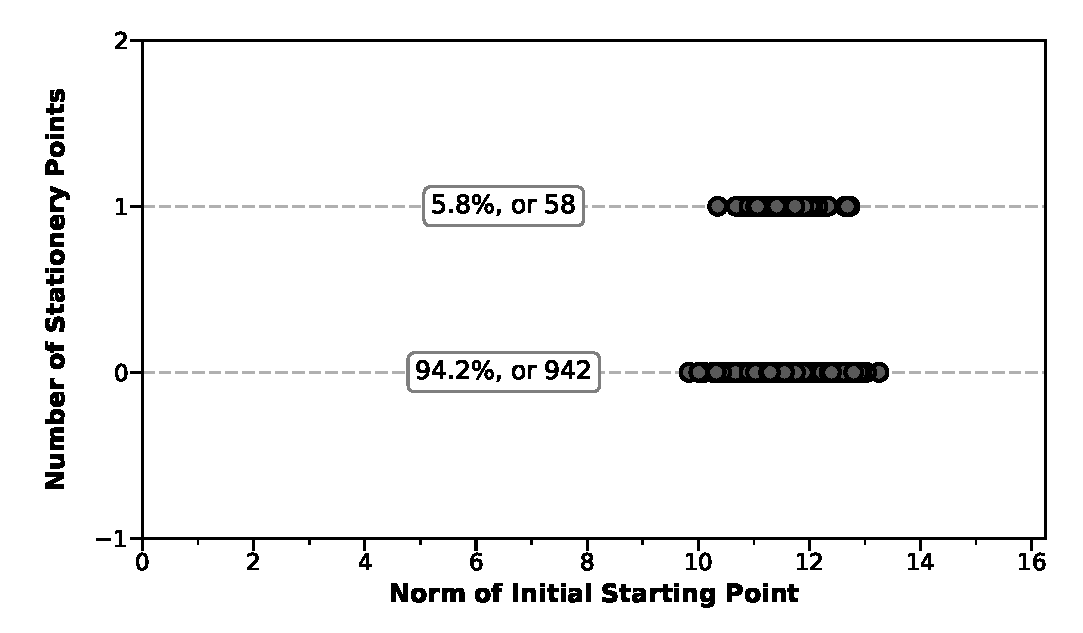
\includegraphics[clip,width=0.7\columnwidth]{./figs/chap4_test/nonconvex_1000_random.eps}%
  \caption{Success Minimizers. \label{fig:nonconvex}}
\end{figure}

Figure ~\ref{fig:nonconvex} shows one sample statistical results for the random study using 
$\epsilon_{\text{krylov}}=10^{-5}$ and $\tau = 10^{-2}$. The plot shows that $94.2\%$ of the $1000$ random cases 
successfully converge to the minimizer, while the rest $5.8\%$ of the $1000$ cases failed in one dimension.    
  
The results show that the optimization method can start from infeasible points, and can handle certain 
amount of nonconvexity. The preconditioner is not used here.  Admittedly, this nonconvex test problem is rather simple, with no complexities like bad-scaling, ill-conditioning included. However, the focus is solely to see whether the added regularization from the homotopy term can help 
Newton's method bypass local maximization points.  Further work is needed to determine when the problem demands 
tighter tolerances and how to detect and handle nonnegative curvature.  

 \subsection{Results - Convergence Plots} 
 
A typical optimization convergence plot is provided in Figure~\ref{fig:nc_converg}. Figure~\ref{fig:ncmu} 
shows the absolute optimality, complementarity and feasibility at each Homotopy iteration of different $\mu$. 
Note that for simplicity, only the Predictor points are displayed when $\mu \geq \epsilon_{\mu}$, 
while the Corrector points are displayed at $\mu < \epsilon_{\mu}$.
Figure~\ref{fig:nccpu} shows convergence plot w.r.t CPU time, 
which is used more often later when the performance of the new method is benchmarked with other 
optimization packages.

\begin{figure}[tbp]
  \centering
  \subfloat[Convergence vs. $\mu$ \label{fig:ncmu}]{
   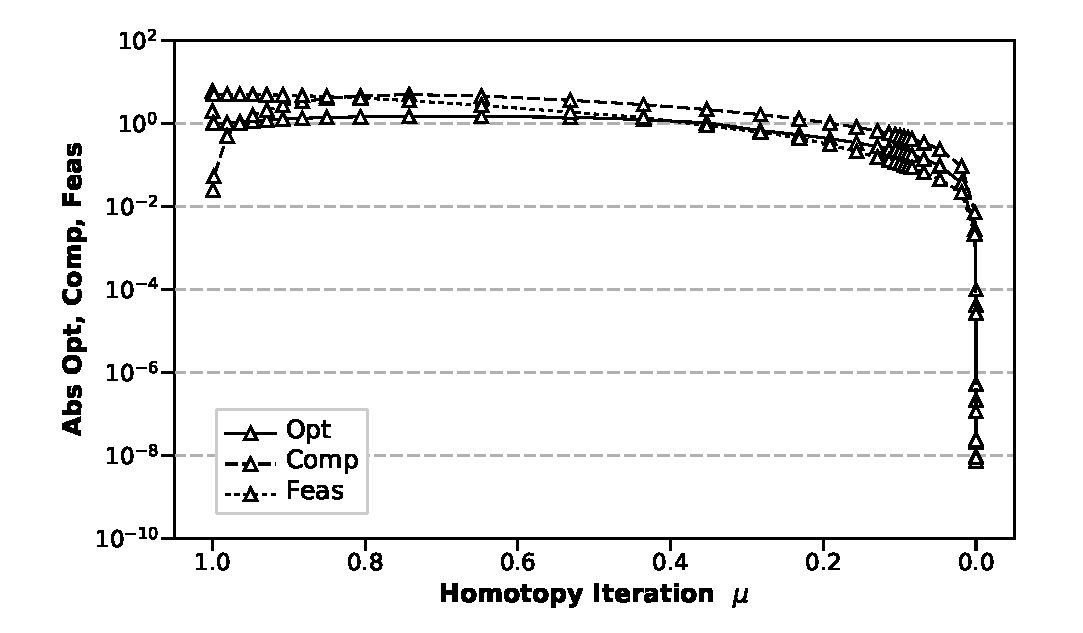
\includegraphics[clip,width=0.7\linewidth]{./figs/chap4_test/nonconvex_mu.eps} }
   \hspace{1em}
   \subfloat[Convergence vs. CPU time \label{fig:nccpu}]{
   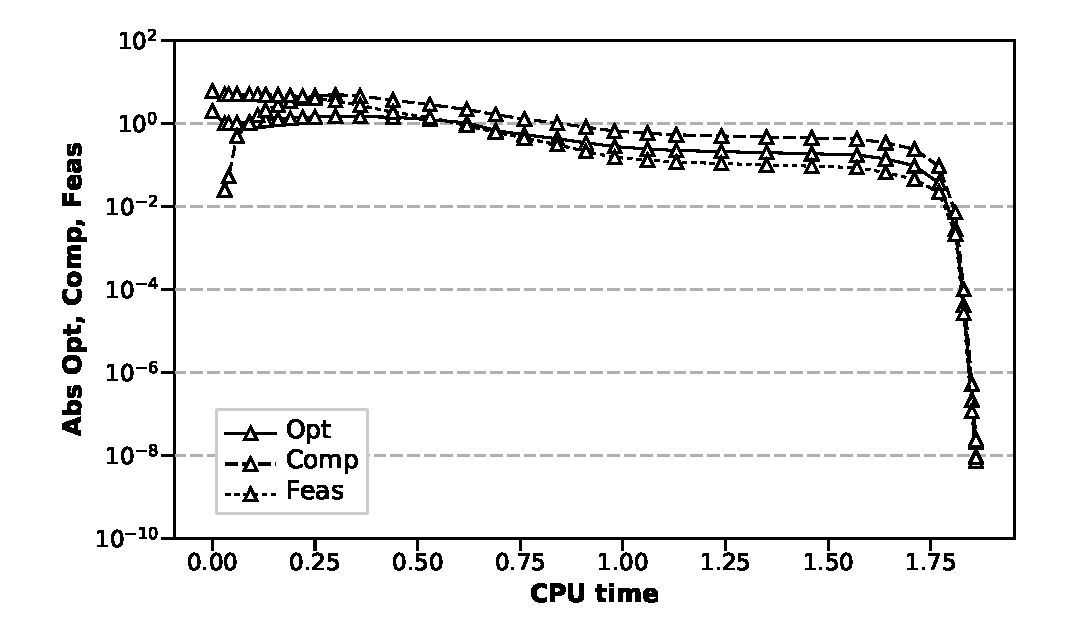
\includegraphics[clip,width=0.7\linewidth]{./figs/chap4_test/nonconvex_cpu.eps} }
   \caption{Typical Convergence Plots in $1000$ Random Cases \label{fig:nc_converg}}
\end{figure}

%\begin{remark}
% The parameters $\alpha_0$, $\delta_{\text{targ}}$, $\phi_{\text{targ}}$, and
%  $\Delta \mu_{\max}$ all play a role in the ability of Algorithm~\ref{alg:pc}
%  to handle nonconvex objectives.  If these parameters are set too agressively,
%  then the algorithm may move off the homotopy level-set and converge to a local
%  maximizer or saddle, even for the simple problem considered here.
%  \padd{I think this Remark should be removed now. As we've provided the influence of 
%  Krylov tolerance and inner tolerance on the success rate. }
%\end{remark}

\section{Scalable quadratic optimization problem}
\subsection{Problem Description}
The next numerical experiement is intended to test the effectiveness of the approximate SVD
preconditioner defined in Algorithm~\ref{alg:precond}.  In particular, we are
interested in the performance of the algorithm with the preconditioner as the size of the problem increases.  
To this end, we consider the following scalable optimization problem
in which we can independently control the size and conditioning of the Hessian
and constraint Jacobian:
\begin{equation}\label{eq:quadra}
  \begin{aligned}
    &\underset{x \in R^n} {\text{min}}  
    & & \frac{1}{2}x^T \mat{Q} x + g^T x \\
    &\text{subject to} & & \mat{A}x \geq b  \\
  \end{aligned}.
\end{equation}
The vectors $g\in \mathbb{R}^{n}$ are randomly sampled from a uniform distribution 
in $[ 0,1)$, while $b \in \mathbb{R}^{n}$ from $[0,0.1)$. 

The Hessian $\mat{Q}$ is diagonal with entries
\begin{equation*}
  \mat{Q}_{ii} = \begin{cases}
    \frac{1}{i}, &  i = 1, 2, ...,  \kappa, \\
    \frac{1}{\kappa}, & i =  \kappa+1, ... , n, \\
  \end{cases}
\end{equation*}
where $\kappa \leq n$.  This definition produces a Hessian with a condition
number of $\kappa$,  so that the condition number
stays the same as the dimension of the problem increases from $100$ to $500$. 

The constraint Jacobian $\mat{A} \in \mathbb{R}^{n\times n}$ is defined as follows. Suppose
$\mat{D} \in \mathbb{R}^{n\times n}$ is a diagonal
matrix of singular values defined similar to $\mat{Q}$:
\begin{equation*}
  \mat{D}_{ii} = \begin{cases}
    \frac{1}{i^2}, &  i = 1,2,...,\nu, \\
    \frac{1}{\nu^2}, & i = \nu+1, ..., n, \\
  \end{cases}
\end{equation*}
where $\nu \leq n$.  Then, $\mat{A}_L $ and $\mat{A}_R$ are matrices of random integers from 
the discrete uniform distribution in the
interval [0,10),  which are applied with $QR$ factorizations,  
\begin{equation*}
\begin{aligned}
\mat{A}_L &= \mat{Q}_L \mat{R}_L \\
\mat{A}_R &= \mat{Q}_R \mat{R}_R \\
\end{aligned}
\end{equation*}
The constraint Jacobian $\mat{A} =\mat{Q}_L  \mat{D} \mat{Q}_R $ 

Consequently, the condition number of $\mat{A}$ is also constant $\nu ^2$ when the dimension 
of the problem increases. 


For this study we chose $\kappa = \nu = 9$, which gives the condition number 
$ \text{cond} (\mat{Q} )= 9$,  $ \text{cond} (\mat{A}) = 81$. The modest condition number of 
$\mat{Q} $ and $\mat{A}$ is benefit to our study in that we can shift 
the focus to treat the ill-condition in the KKT matrix 
$\nabla_{q} F(q)$ at $\mu<\epsilon_{\mu}$, whose typical condition number ranges from $10^4$ to $10^9$
depends on the problem.

The values of $\kappa$ and $\nu$ are chosen to be a fixed positive
value smaller than the number of design variables.  This is to make the
condition number of the matrix fixed, not hugely increasing with the
dimension of the problem.

\begin{remark}
Although the matrices for this synthetic problem are available explicitly, our
algorithm does not exploit this and remains matrix-free, \ie it only uses
matrix-vector products.
\end{remark}

\subsection{Results}
Figure~\ref{fig:quad_hist} plots the absolute optimality, complementarity and feasibility
histories versus CPU time. 
The predictor-corrector algorithm is applied both with and without the preconditioner.  
In addition, the plots include the results
from SNOPT~\cite{gill:2002}, a well-validated active-set SQP
optimization library.

Without the preconditioner, the predictor-corrector algorithm is not competitive
and does not converge after sufficient time.  This illustrates the need for preconditioning Newton-Krylov
optmization algorithms, even for modest sized problems.  The results
also indicate that the proposed algorithm outperforms SNOPT on this particular
problem.  SNOPT is able to establish feasiblity within the same time as the
predictor-corrector algorithm, but it takes significantly longer to converge the
first-order optimality conditions.

\begin{figure}[tbp]
  \centering
  \subfloat[$n=200$\label{fig:quad_200}]{
   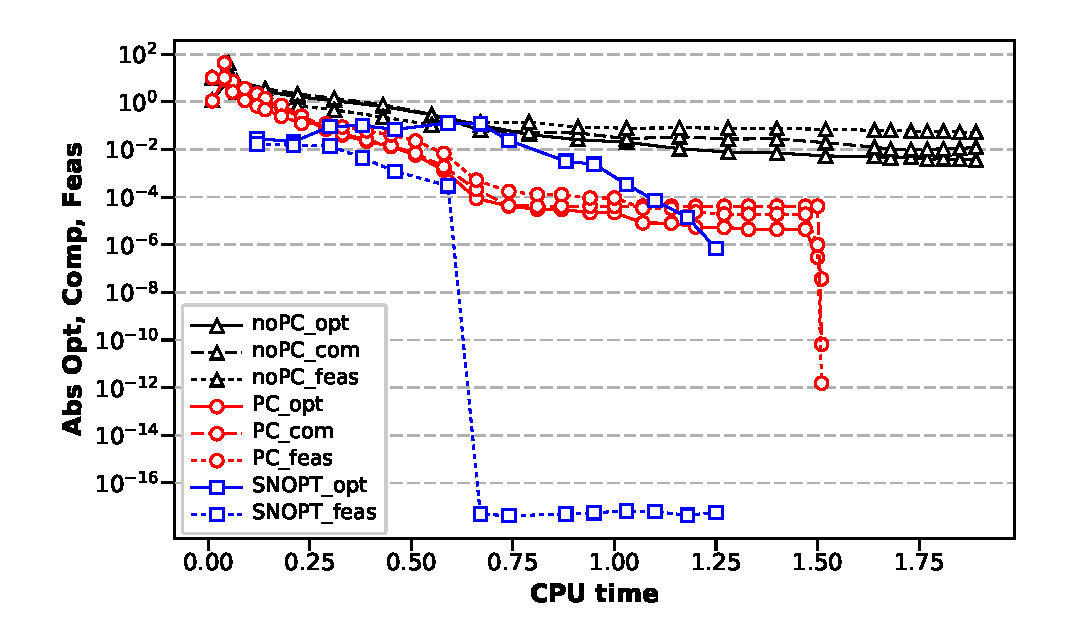
\includegraphics[clip,width=0.7\linewidth]{./figs/chap4_test/quadratic_200_color.eps} }
   \hspace{1em}
   \subfloat[$n=500$\label{fig:quad_500}]{
   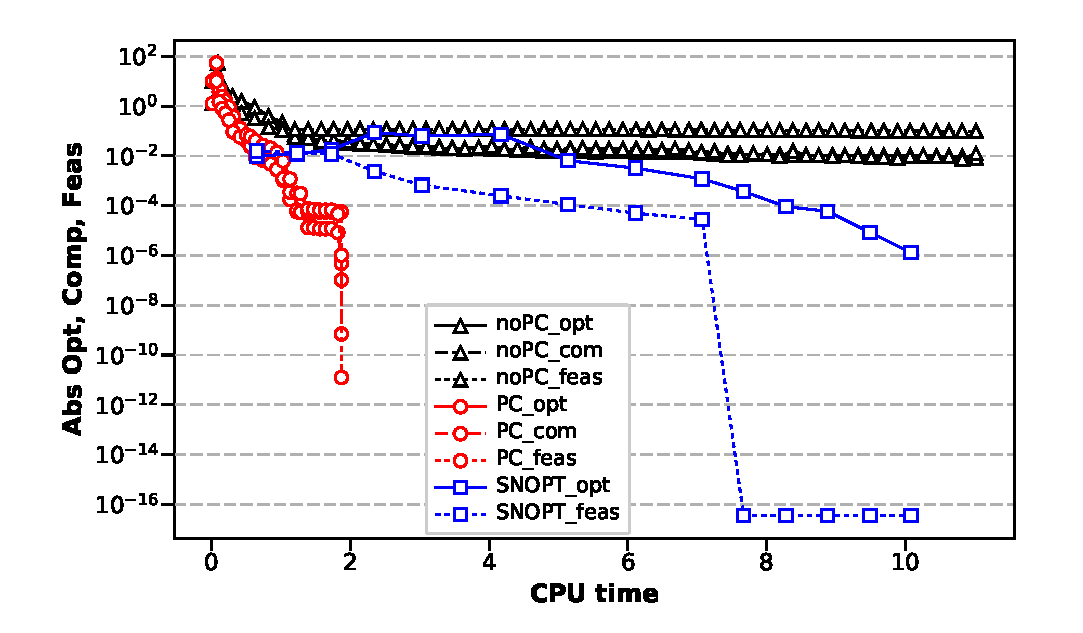
\includegraphics[clip,width=0.7\linewidth]{./figs/chap4_test/quadratic_500_color.eps} }
   \caption{Convergence histories for the quadratic problem with $n=200$ and
  $n=500$. The results for the proposed algorithm, with and without
  preconditioning, are plotted together with the results from
  SNOPT.\label{fig:quad_hist}}
\end{figure}

To further explore the scalability of the proposed algorithm, we run 100 random cases for 
each fixed sized problem, for $n = 100, 200, 300, 400, 500$.  In each random case, the gradient 
in the objective function $g$, and the right hand side vector $b$ in the linear constraint in \eqref{eq:quadra} 
are randomly generated. The diagonal Hessian $\mat{Q}$ and $\mat{D}$ is fixed, while $\mat{A}_L$ and $\mat{A}_R$ are randomly generated. So the constraint Jacobian $\mat{A}$ is also changing. The starting point for each run is also randomly generated. Figure~\ref{fig:quad_scale} shows the error bar of the CPU time while
the problem size increases. As can be seen, the new method exhibits good scalability performances, in comparison with SNOPT. 

\begin{figure}[tbp]
  \centering
  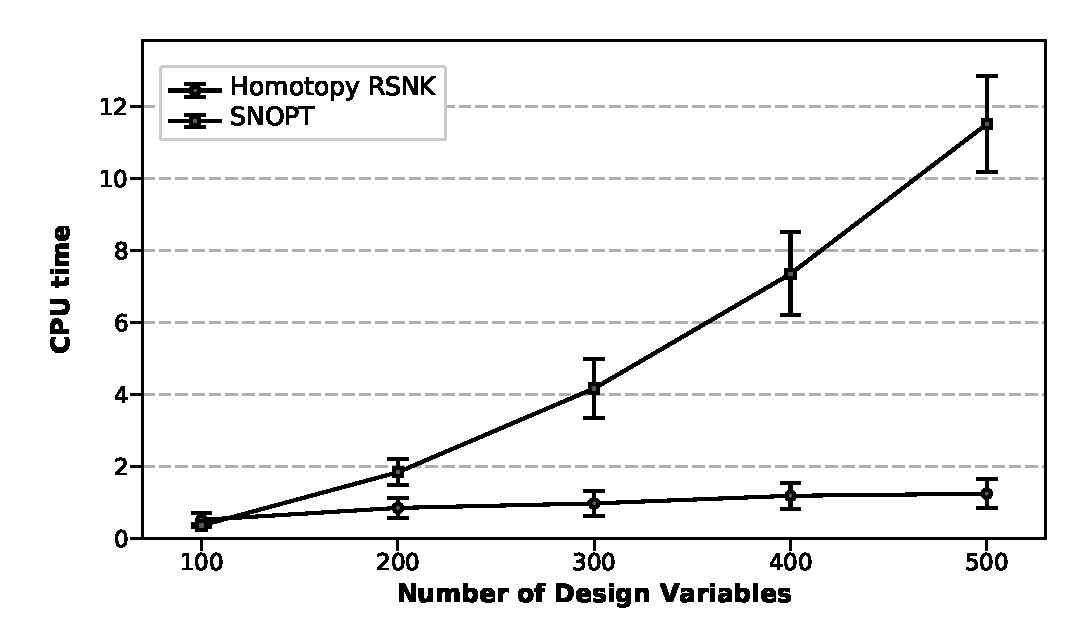
\includegraphics[clip,width=0.8\textwidth]{./figs/chap4_test/quadratic_random_100_nocolor.eps}%
  \caption{CPU cost versus number of design variables for the quadratic
    optimization problem.\label{fig:quad_scale}}
\end{figure}

It is worthwhile to emphasize that the proposed SVD preconditioner is particularly effective for this constructed problem, because the problem is designed in such a way that the distribution of the singular values for the constraint Jacobian is readily separable, with the largest few dominates, and there are only linear inequality constraints. Put another way, SVD approximation can capture the main characteristics of the matrix in~\eqref{eq:svd}. For real-world problems, the distribution of the singular values of the constraint Jacobian is unknown, and may possess unfavorable distribution patterns. The the proposed preconditioner may not be as effective.  




